\begin{frame}{$hp$-FEM}
  {Definition}
  \tiny
  "The \alert{$hp$-FEM} is a general version of the finite element method (FEM), a numerical method for solving partial differential equations based on piecewise-polynomial approximations that employs elements of variable size ($h$) and polynomial degree ($p$).  The origins of $hp$-FEM date back to the pioneering work of Ivo Babuska who discovered that the finite element method \alert{converges exponentially fast when the mesh is refined using a suitable combination of $h$-refinements} (dividing elements into smaller ones) \alert{and $p$-refinements} (increasing their polynomial degree).  The exponential convergence makes the method a very attractive choice compared to most other finite element methods which only converge with an algebraic rate.  The exponential convergence of the $hp$-FEM was not only predicted theoretically but also observed by numerous independent researchers." [Wikipedia]

\end{frame}

\begin{frame}{$hp$-FEM}
  \footnotesize
  
  \begin{block}{Hermes Project}
Hermes is a C++ library for rapid development of $hp$-FEM solvers.  The library is currently developed by Pavel Solin's group at the University of Nevada, Reno (UNR), and their collaborators from numerous places around the globe.
  \end{block}
\vspace{.3cm}

Hermes provides
\begin{itemize}
\item mature $hp$-adaptivity algorithms
\item wide applicability
\item arbitrary level hanging nodes
\item multimesh $hp$-FEM
\end{itemize}

\end{frame}

%%%%%%%%%%%%%%%%%%%%%%%%%%%%%%%%%%%%%%%%%%%%%%%%

\begin{frame}{$hp$-FEM}
  {Understanding the convergence rates}
  
  \scriptsize

    When using elements of degree $ p $ we expect a slope of $ - p/d $ on the log-log scale
    
    ($ d $ is the dimension)

    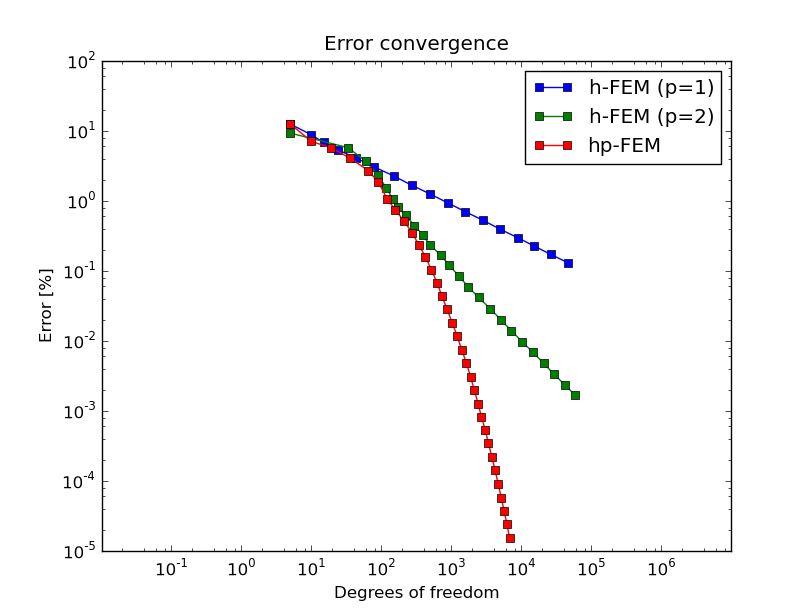
\includegraphics[width=6cm]{figures/conv_dof15}
    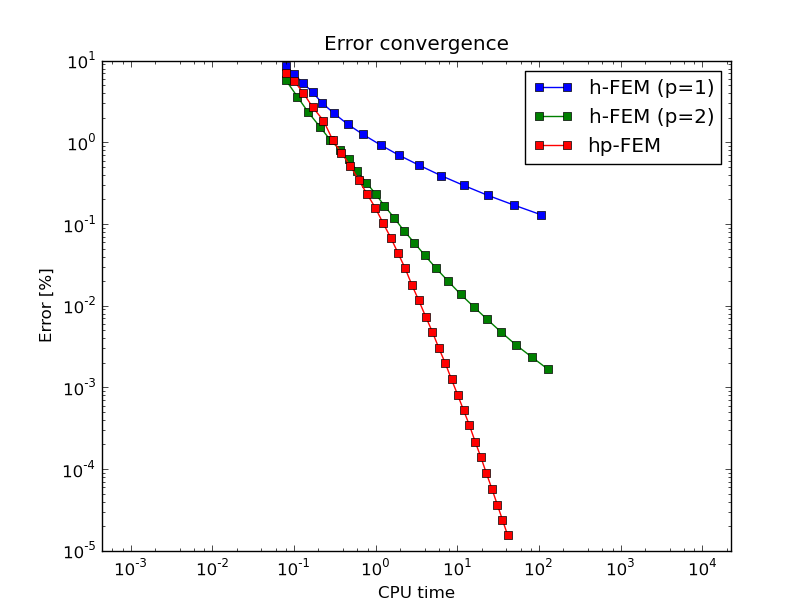
\includegraphics[width=6cm]{figures/conv_cpu15}
    

\end{frame}

%%%%%%%%%%%%%%%%%%%%%%%%%%%%%%%%%%%%%%%%%%%%%%%%

\begin{frame}{$hp$-FEM}
  {Adaptivity in the $hp$-FEM and in Hermes}
  
  \begin{columns}
  \begin{column}{5cm}
    \tiny
    An element can be refined in many different ways

     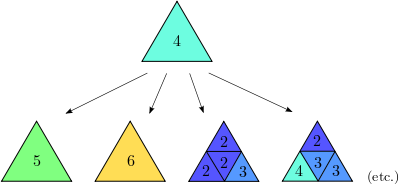
\includegraphics[width=5cm]{figures/refinements}
     
     \vspace{.3cm}
     
     Number of refinement candidates relatively low in $ h $ or $ p $ adaptivity, much higher in $ hp $ adaptivity
      
     %The number of possible element refinements is implementation-dependent.   In general it is very low in $ h $ or $ p $ adaptivity, much higher in $ hp $ adaptivity, and it rises even more when anisotropic refinements are enabled.

  \end{column}
  \begin{column}{7cm}
  \scriptsize  
  \begin{block}{Automatic adaptivity in Hermes}
    \begin{enumerate}
    \item Generate refinement candidates
    \item Estimates local errors by projecting reference solution onto FE spaces
    \item Calculate number of degree of freedom (DOF) contributed by each candidate
    \item Calculates a score for each candidate, and sort them according to their scores
    \item Select candidate with highest score
    \end{enumerate}
  \end{block}

    By default in Hermes, the score is $ s = \frac{\log_{10} e_{0} - \log_{10} e}{(d_{0} - d)^{\xi}} $
    %where $ e $ and $ d $ are an estimated error and an estimated number of DOF of a candidate respectively, $ e_0 $ and $ d_0 $ are an estimated error and an estimated number of DOF of the examined element respectively, and $ \xi $ is a convergence exponent
    
    %and the error estimate is calculated as $ e = \frac{\|u-u_{ref}\|_{H^{1}}}{\|u_{ref}\|_{H^{1}}} $

  \end{column}
  \end{columns}

\end{frame}



\begin{frame}{$hp$-FEM}
  {Multimesh}

   \tiny
   (A) is the master mesh, (B) - (D) three different meshes, and (E) is the virtual union mesh
    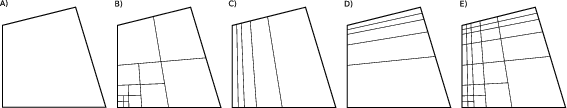
\includegraphics[width=8cm]{figures/multimesh}

    \vspace{.3cm}

    The union mesh is not constructed physically in the computer memory -- it merely serves as a "hint" to correctly transform integration points while integrating over sub-elements of the elements of the existing meshes

    %The following figure shows the integration over an element  of the virtual union mesh, and what are the appropriate subelements of the existing elements where this integration is performed
    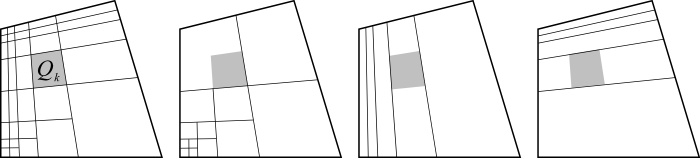
\includegraphics[width=8cm]{figures/multimesh2}

    %The adaptivity procedure for single PDE could be extended directly to systems of PDEs.  In this way, error estimates in $ H^{1} $ norm are calculated for elements in both spaces independently and the worst ones are refined. However, this approach is not optimal if the PDEs are coupled, since an error caused in one solution component influences the errors in other components and vice versa.

    %Recall that in elliptic problems the bilinear form $ a(u, v) $ defines the energetic inner product, $ (u, v)_{e} = a(u, v) $.

    %The norm induced by this product $ \|u\|_{e} = \sqrt{(u, u)_{e})} $, is called the energy norm. When measuring the error in the energy norm of the entire system, one can reduce the above-mentioned difficulties dramatically. When calculating the error on an element, the energy norm accounts also for the error caused by other solution components.

%The adaptivity algorithm does not make distinctions between various meshes. The elements of all meshes in the system are put into one single array, sorted according to their estimated errors, and then the ones with the largest error are refined. In other words, it may happen that all elements marked for refinement will belong just to one mesh.

\end{frame}

\begin{frame}{$hp$-FEM}
  {Example with Hermes2D}
  \tiny
  \begin{columns}
  \begin{column}{5cm}
    We consider a simplified Fitzhugh-Nagumo system
      
    $ -d_u^2 \Delta u - f(u) + \sigma v = g_1 $

    $ -d_v^2 \Delta v - u + v = g_2 $
    
    \vspace{.3cm}

    In the original equation, $ f(u) = \lambda u - u^3 - \kappa $.  For simplicity, here we just take $ f(u) = u $.

    Domain: Square $ (-1,1)^2 $.
    
    BC: Both solution components are zero on the boundary.
 

    %The following two figures show the solutions $ u $ and $ v $.  Notice their large qualitative differences: While $ u $ is smooth in the entire domain, $ v$ has a thin boundary layer along the boundary:
    \hspace{0.5cm} 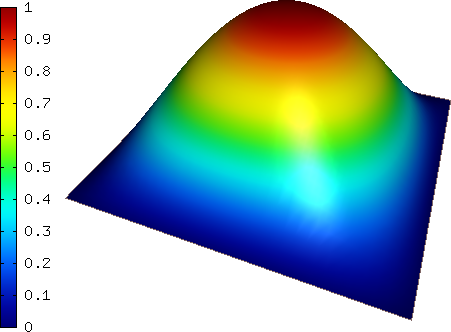
\includegraphics[width=3cm]{figures/solution_u}
    
    \hspace{1.5cm} 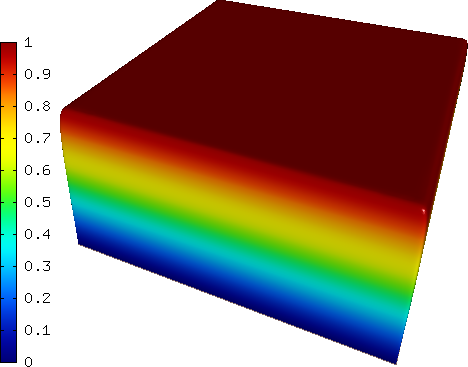
\includegraphics[width=3cm]{figures/solution_v}

  \end{column}
  \begin{column}{7cm}
     
    Exact solution: The functions $g_1$ and $g_2$ were calculated so that the exact solution is
    $ u(x,y) = \cos(\frac{\pi x}{2}) \cos(\frac{\pi y}{2}) $
    
    $ v(x,y) = \left[1 - \frac{(\exp(k x)+\exp(-k x))}{(\exp(k) + exp(-k)}\right] \left[1 - \frac{(\exp(k y)+\exp(-k y))}{(\exp(k) + exp(-k)}\right] $
  
    \vspace{.3cm}
  
    Resulting mesh for $ u $ and $ v $ obtained using conventional (single-mesh) hp-FEM: 12026 DOF (6013 for each solution)
    
    Resulting mesh for $ u $ obtained using the multimesh hp-FEM: 169 DOF
    
    Resulting mesh for $ v $ obtained using the multimesh hp-FEM: 3565 DOF
    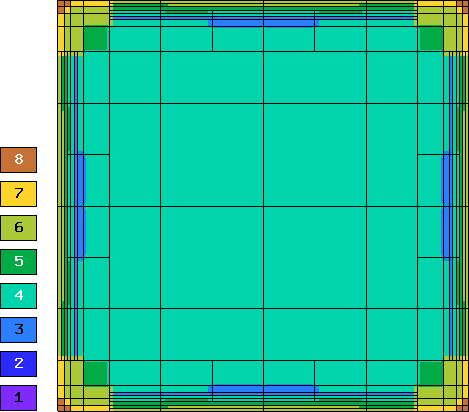
\includegraphics[width=2.3cm]{figures/mesh_single}
    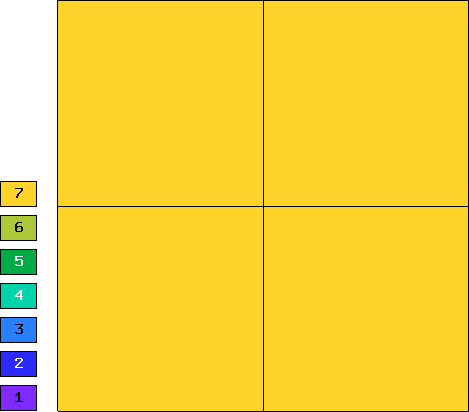
\includegraphics[width=2.3cm]{figures/mesh_multi_u}
    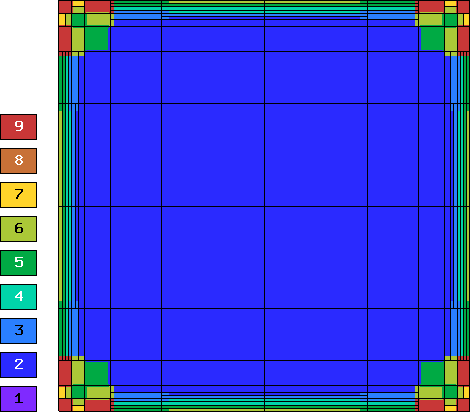
\includegraphics[width=2.3cm]{figures/mesh_multi_v}

    DOF and CPU convergence graphs:
    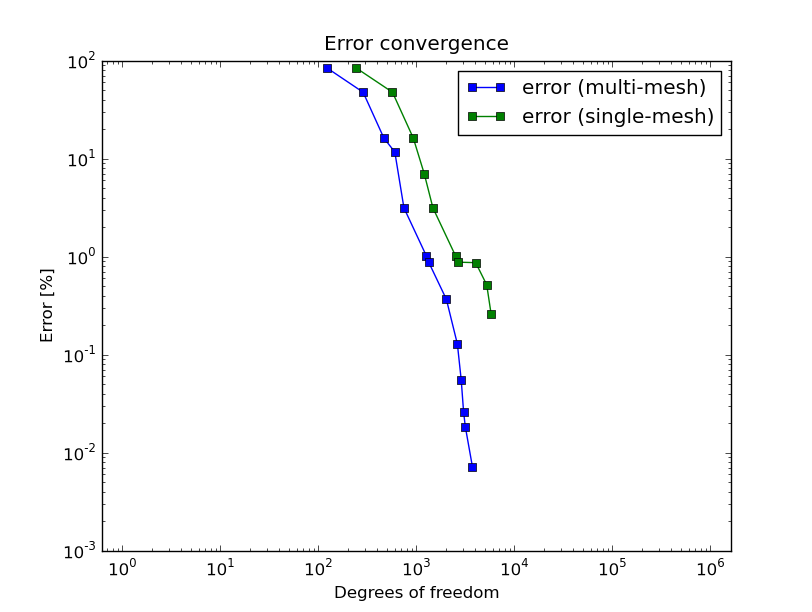
\includegraphics[width=3.5cm]{figures/conv_dof12}
    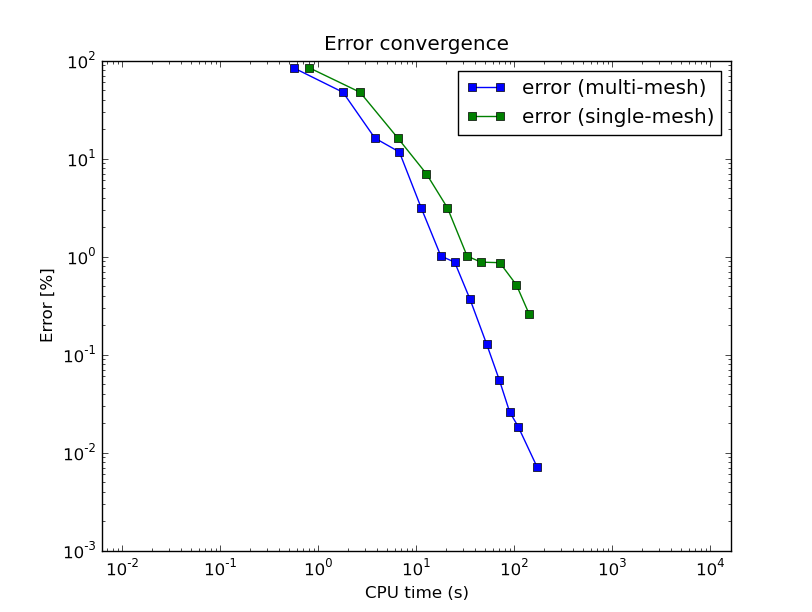
\includegraphics[width=3.5cm]{figures/conv_cpu12}
    
  \end{column}
  \end{columns}

\end{frame}
